\begin{frame}{Quantification: Rappel}
    \centering
    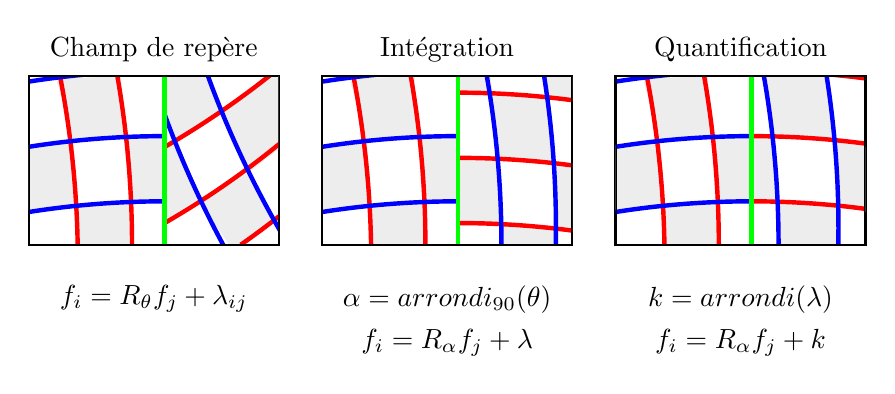
\begin{tikzpicture}[scale=1.38]
		\begin{scope}
			\draw[thick] (-.35, 0) -- (1.95, 0) -- (1.95, 1.55) -- (-.35, 1.55) -- cycle;
			\clip (-.35, 0) -- (1.95, 0) -- (1.95, 1.55) -- (-.35, 1.55) -- cycle;
			\fill[gray!14] (.06, .97) -- (.53, 1) -- (.5, 1.55) -- (-.1, 1.53);
			\fill[gray!14] (.06, .97) -- (-.5, .9) -- (-.5, .3) -- (.1, .37);
			\fill[gray!14] (.1, .37) -- (.57, .4) -- (.58, 0) -- (.1, 0);
			\fill[gray!14] (.57, .4) -- (.9, .4) -- (.9, 1.) -- (.53, 1.);
			\fill[gray!14] (.9, 1.2) -- (.9, 1.55) -- (1.3, 1.55) -- (1.44, 1.24) -- (.98, .96);
			\fill[gray!14] (1.44, 1.24) -- (1.95, 1.6) -- (1.95, .88) -- (1.68, .67);
			\fill[gray!14] (.9, .9) -- (.99, .98) -- (1.2, .42) -- (.9, .22);
			\fill[gray!14] (1.53, -.05) -- (1.2, .42) -- (1.68, .67) -- (1.9, .22);
			\draw[ultra thick, red] (0.1, 0) arc(1:11:9);
			\draw[ultra thick, red] (.6, 0) arc(0:10:9);
			\draw[ultra thick, blue] (.9, 0.4) arc(90:99:8);
			\draw[ultra thick, blue] (.9, 1) arc(90:99:8);
			\draw[ultra thick, blue] (.9, 1.6) arc(90:99:8);
			\draw[ultra thick, red] (.9, .2) arc(-60:-50:8);
			\draw[ultra thick, red] (.9, .9) arc(-60:-51:8);
			\draw[ultra thick, red] (1.6, 0) arc(-55:-51:8);
			\draw[ultra thick, blue] (.9, 1.2) arc(200:209:9);
			\draw[ultra thick, blue] (1.3, 1.55) arc(200:210:9);
			\draw[ultra thick, green] (.9, 0) -- (.9, 1.55);
			\draw[thick] (-.35, 0) -- (1.95, 0) -- (1.95, 1.55) -- (-.35, 1.55) -- cycle;
		\end{scope}
		\node at (.8, 1.8) {Champ de repère};
		\node at (.8, -0.5) {$f_i = R_{\theta} f_j + \lambda_{ij}$};
		\begin{scope}[xshift=2.7cm]
			\draw[thick] (-.35, 0) -- (1.95, 0) -- (1.95, 1.55) -- (-.35, 1.55) -- cycle;
			\clip (-.35, 0) -- (1.95, 0) -- (1.95, 1.55) -- (-.35, 1.55) -- cycle;
			\fill[gray!14] (.06, .97) -- (.53, 1) -- (.5, 1.55) -- (-.1, 1.53);
			\fill[gray!14] (.06, .97) -- (-.5, .9) -- (-.5, .3) -- (.1, .37);
			\fill[gray!14] (.1, .37) -- (.57, .4) -- (.58, 0) -- (.1, 0);
			\fill[gray!14] (.57, .4) -- (.9, .4) -- (.9, 1.) -- (.53, 1.);
			\fill[gray!14] (.9, .2) -- (.9, .8) -- (1.27, .78) -- (1.29, .17);
			\fill[gray!14] (1.8, .16) -- (1.77, .76) -- (1.95, .75) -- (1.95, .12);
			\fill[gray!14] (1.27, .78) -- (1.77, .76) -- (1.74, 1.36) -- (1.22, 1.38);
			\fill[gray!14] (.9, 1.4) -- (1.22, 1.39) -- (1.2, 1.55) -- (.9, 1.55);
			\fill[gray!14] (1.73, 1.34) -- (1.71, 1.55) -- (1.95, 1.55) -- (1.95, 1.32);
			\fill[gray!14] (1.3, 0) -- (1.8, 0) -- (1.8, .14) -- (1.3, .18);
			\draw[ultra thick, red] (0.1, 0) arc(1:11:9);
			\draw[ultra thick, red] (.6, 0) arc(0:10:9);
			\draw[ultra thick, blue] (.9, 0.4) arc(90:99:8);
			\draw[ultra thick, blue] (.9, 1) arc(90:99:8);
			\draw[ultra thick, blue] (.9, 1.6) arc(90:99:8);
			\draw[ultra thick, red] (.9, .2) arc(90:82:8);
			\draw[ultra thick, red] (.9, .8) arc(90:82:8);
			\draw[ultra thick, red] (.9, 1.4) arc(90:82:8);
			\draw[ultra thick, blue] (1.3, 0) arc(0:10:9);
			\draw[ultra thick, blue] (1.8, 0) arc(-1:9:9);
			\draw[ultra thick, green] (.9, 0) -- (.9, 1.55);
			\draw[thick] (-.35, 0) -- (1.95, 0) -- (1.95, 1.55) -- (-.35, 1.55) -- cycle;
		\end{scope}
		\node at (3.5, 1.8) {Intégration};
		\node at (3.5, -0.5) {\green{$\alpha = arrondi_{90}(\theta)$}};
		\node at (3.5, -.9) {$f_i = R_{\green{\alpha}} f_j + \lambda$};
		
		\begin{scope}[xshift=5.4cm]
			\draw[thick] (-.35, 0) -- (1.95, 0) -- (1.95, 1.55) -- (-.35, 1.55) -- cycle;
			\clip (-.35, 0) -- (1.95, 0) -- (1.95, 1.55) -- (-.35, 1.55) -- cycle;
			\fill[gray!14] (.06, .97) -- (.53, 1) -- (.5, 1.55) -- (-.1, 1.53);
			\fill[gray!14] (.06, .97) -- (-.5, .9) -- (-.5, .3) -- (.1, .37);
			\fill[gray!14] (.1, .37) -- (.57, .4) -- (.58, 0) -- (.1, 0);
			\fill[gray!14] (.57, .4) -- (1.13, .4) -- (1.11, 1.) -- (.53, 1.);
			\fill[gray!14] (1.13, .4) -- (1.7, .36) -- (1.7, 0) -- (1.15, 0);
			\fill[gray!14] (1.11, 1.) -- (1.68, .96) -- (1.6, 1.55) -- (1.04, 1.55);
			\fill[gray!14] (1.68, .96) -- (1.95, .9) -- (1.95, .3) -- (1.7, .36);
			\draw[ultra thick, red] (0.1, 0) arc(1:11:9);
			\draw[ultra thick, red] (.6, 0) arc(0:10:9);
			\draw[ultra thick, blue] (.9, 0.4) arc(90:99:8);
			\draw[ultra thick, blue] (.9, 1) arc(90:99:8);
			\draw[ultra thick, blue] (.9, 1.6) arc(90:99:8);
			\draw[ultra thick, red] (.9, .4) arc(90:82:8);
			\draw[ultra thick, red] (.9, 1.) arc(90:82:8);
			\draw[ultra thick, red] (.9, 1.6) arc(90:80:8);
			\draw[ultra thick, blue] (1.15, 0) arc(0:10:9);
			\draw[ultra thick, blue] (1.7, 0) arc(-1:9:9);
			\draw[ultra thick, green] (.9, 0) -- (.9, 1.55);
			\draw[thick] (-.35, 0) -- (1.95, 0) -- (1.95, 1.55) -- (-.35, 1.55) -- cycle;
		\end{scope}
		\node at (6.2, 1.8) {Quantification};
		\node at (6.2, -.5) {\purple{$k = arrondi(\lambda)$}};
		\node at (6.2, -0.9) {$f_i = R_{\green{\alpha}} f_j + \purple{k}$};
	
	\end{tikzpicture}
    \begin{itemize}
        \item Chaque bord devient une valeur entière pour $\blue{u}$ ou $\red{v}$
        \item Chaque découpe devient une translation entière pour $\blue{u}$ et $\red{v}$
        \item Chaque singularité est une valeur entière pour $\blue{u}$ et pour $\red{v}$
		\item La paramétrisation $f = (\blue{u}, \red{v})$ doit rester bijective
    \end{itemize}
\end{frame}

\begin{frame}{Travail inspiré par: Quantized Global Parametrization}
    \centering
    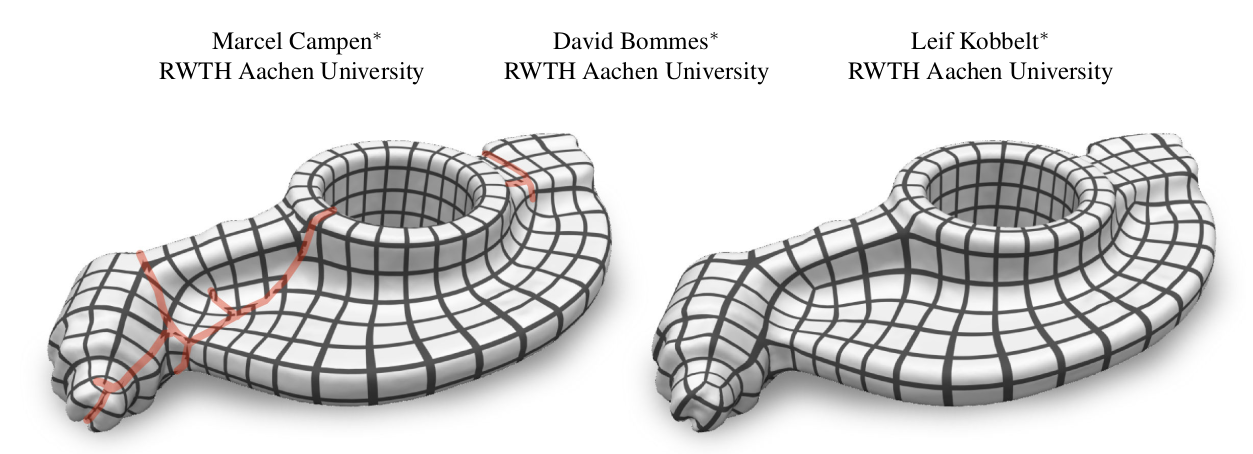
\includegraphics[width=\linewidth]{yoimg/qgp.png}
\end{frame}

\begin{frame}{QGP, Campen et al. 2015}
    \centering
    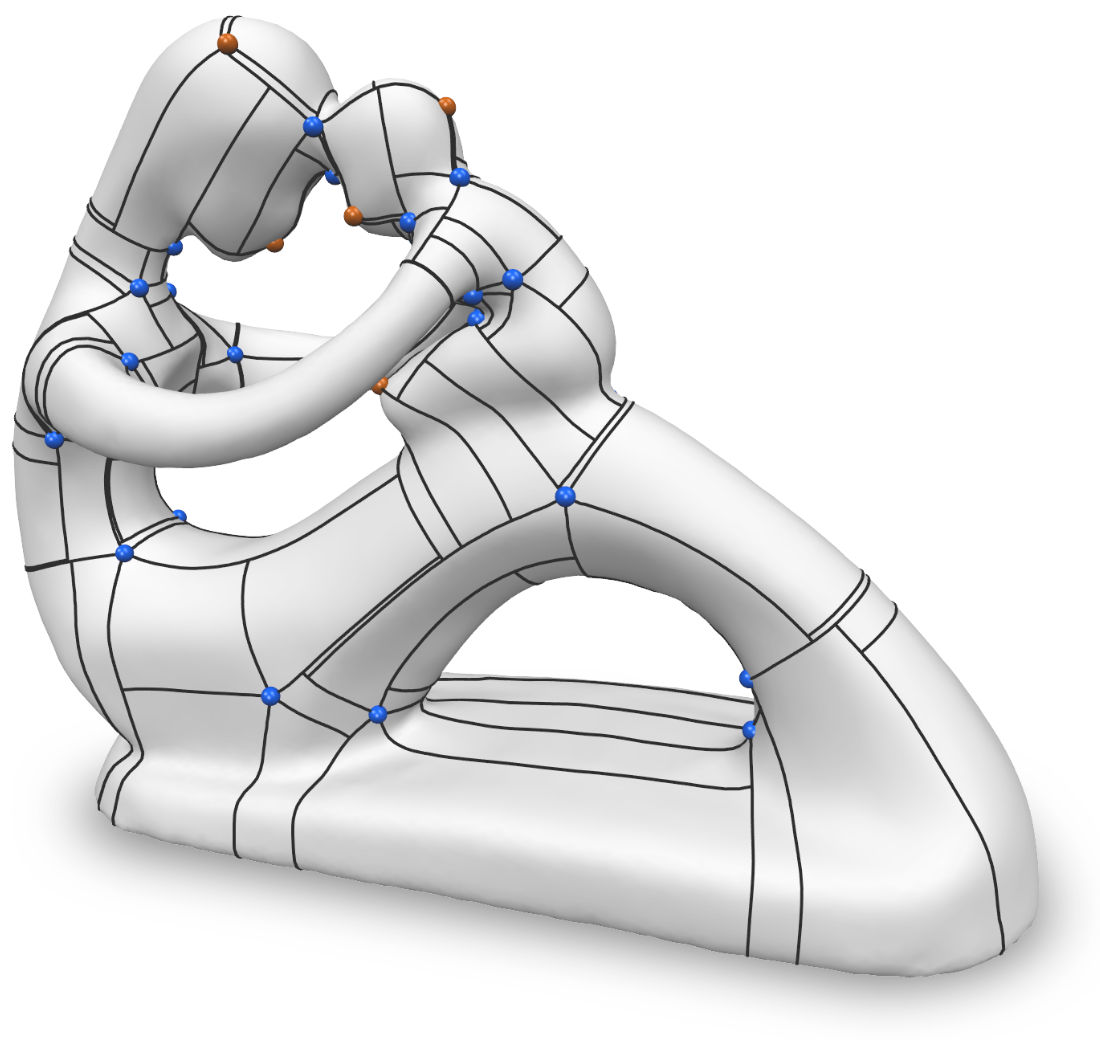
\includegraphics[width=0.48\linewidth]{yoimg/tmesh.png}
    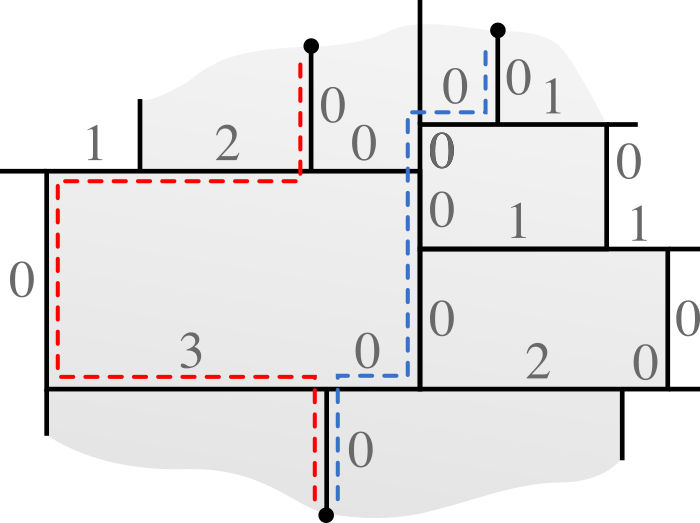
\includegraphics[width=0.42\linewidth]{yoimg/tmesh2.png} \\
    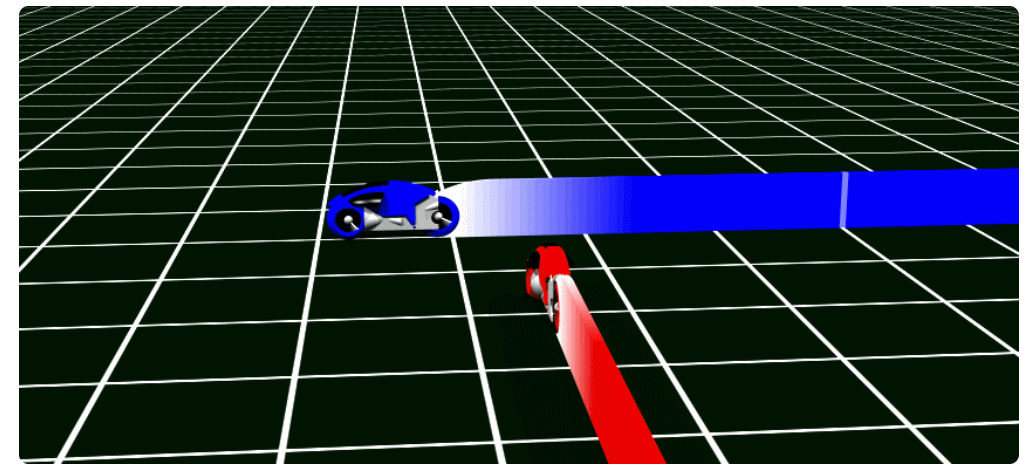
\includegraphics[width=0.33\linewidth]{yoimg/tron.png}
    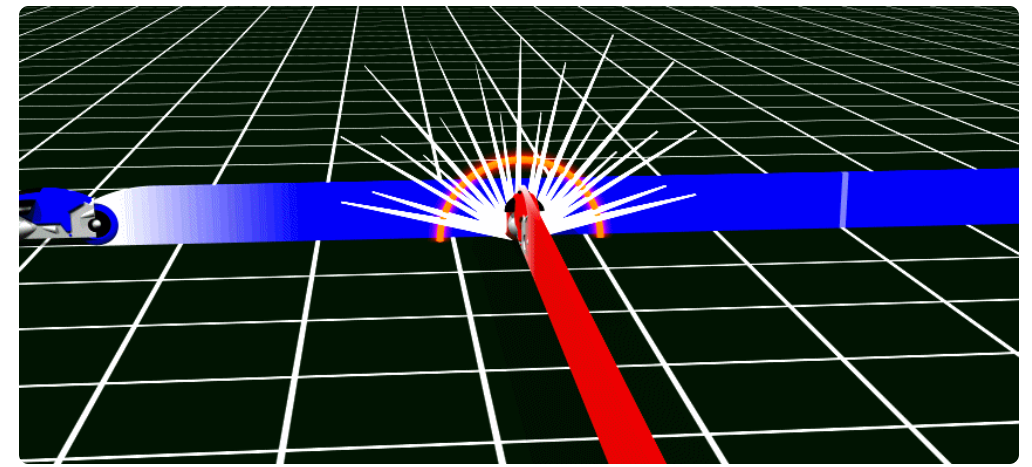
\includegraphics[width=0.33\linewidth]{yoimg/tron2.png}
\end{frame}

\begin{frame}{Contribution: Quantification sans maillage en T}
    \centering
    \small Y. Coudert-\,-Osmont$^1$, D. Desobry$^1$, M. Heistermann$^2$, D. Bommes$^2$, N.Ray$^1$, D. Sokolov$^1$ \\
    \tiny $^1$Inria Nancy - Grand Est, LORIA, France \\
    \tiny $^2$University of Bern, Switzerland \\[2mm]
    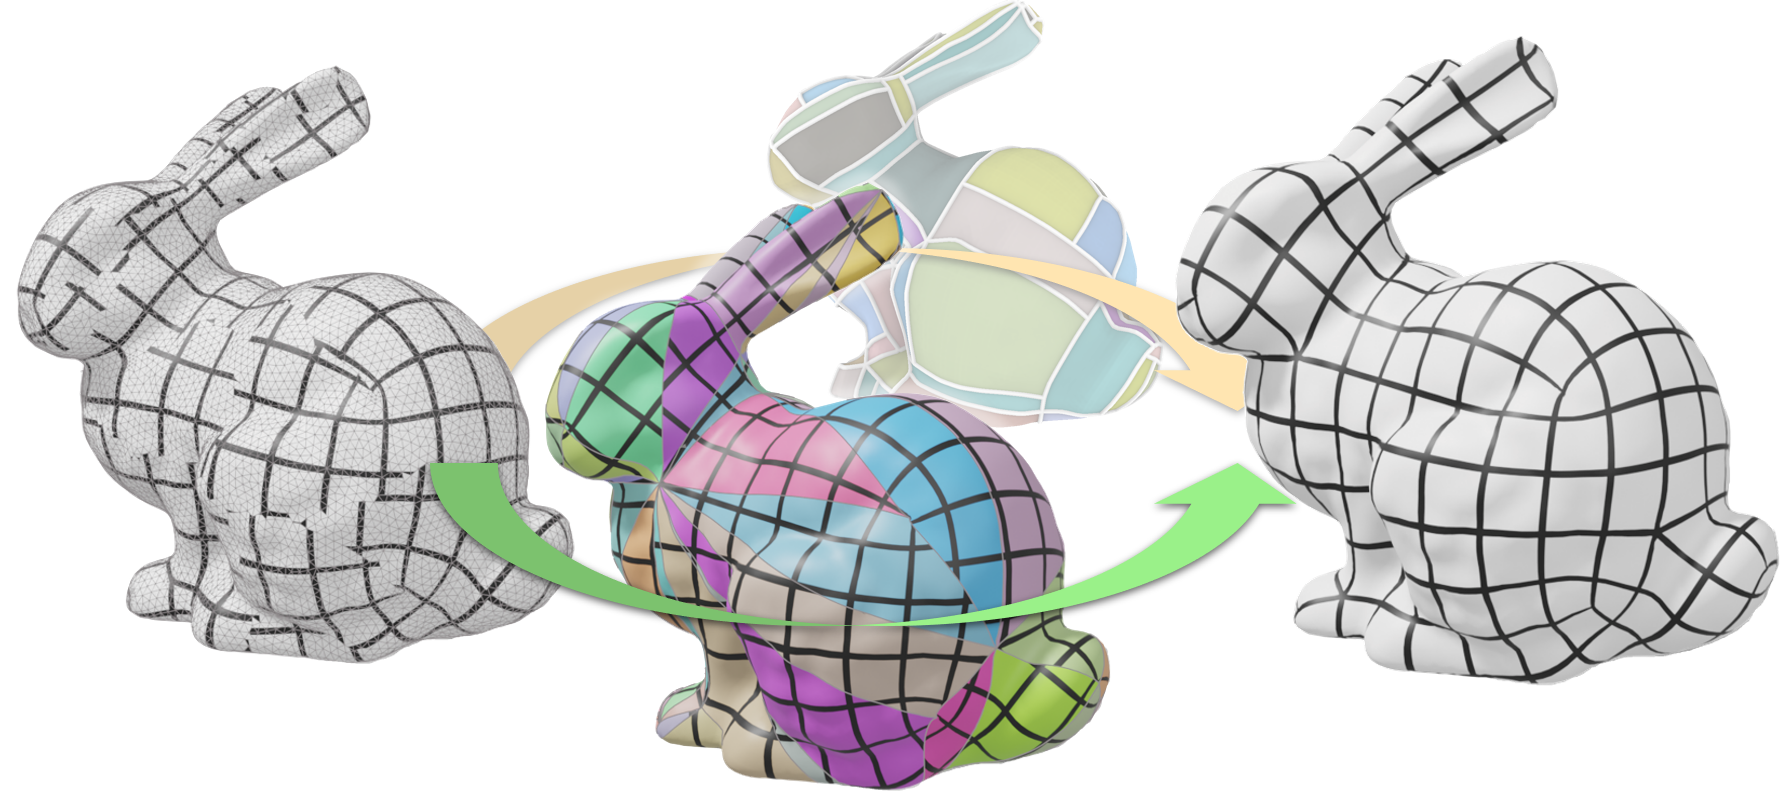
\includegraphics[width=.9\linewidth]{yoimg/teaser.PNG}
\end{frame}

\begin{frame}{Contribution: Quantification sans maillage en T}
    \begin{itemize}
        \item QGP peut écraser des éléments, forçant un recalcul de carte complet, qui peut échouer.\\
        \item Tous nos éléments restent valides, la carte préservant la grille peut être déposée directement sur le maillage initial.\\
        \centering
        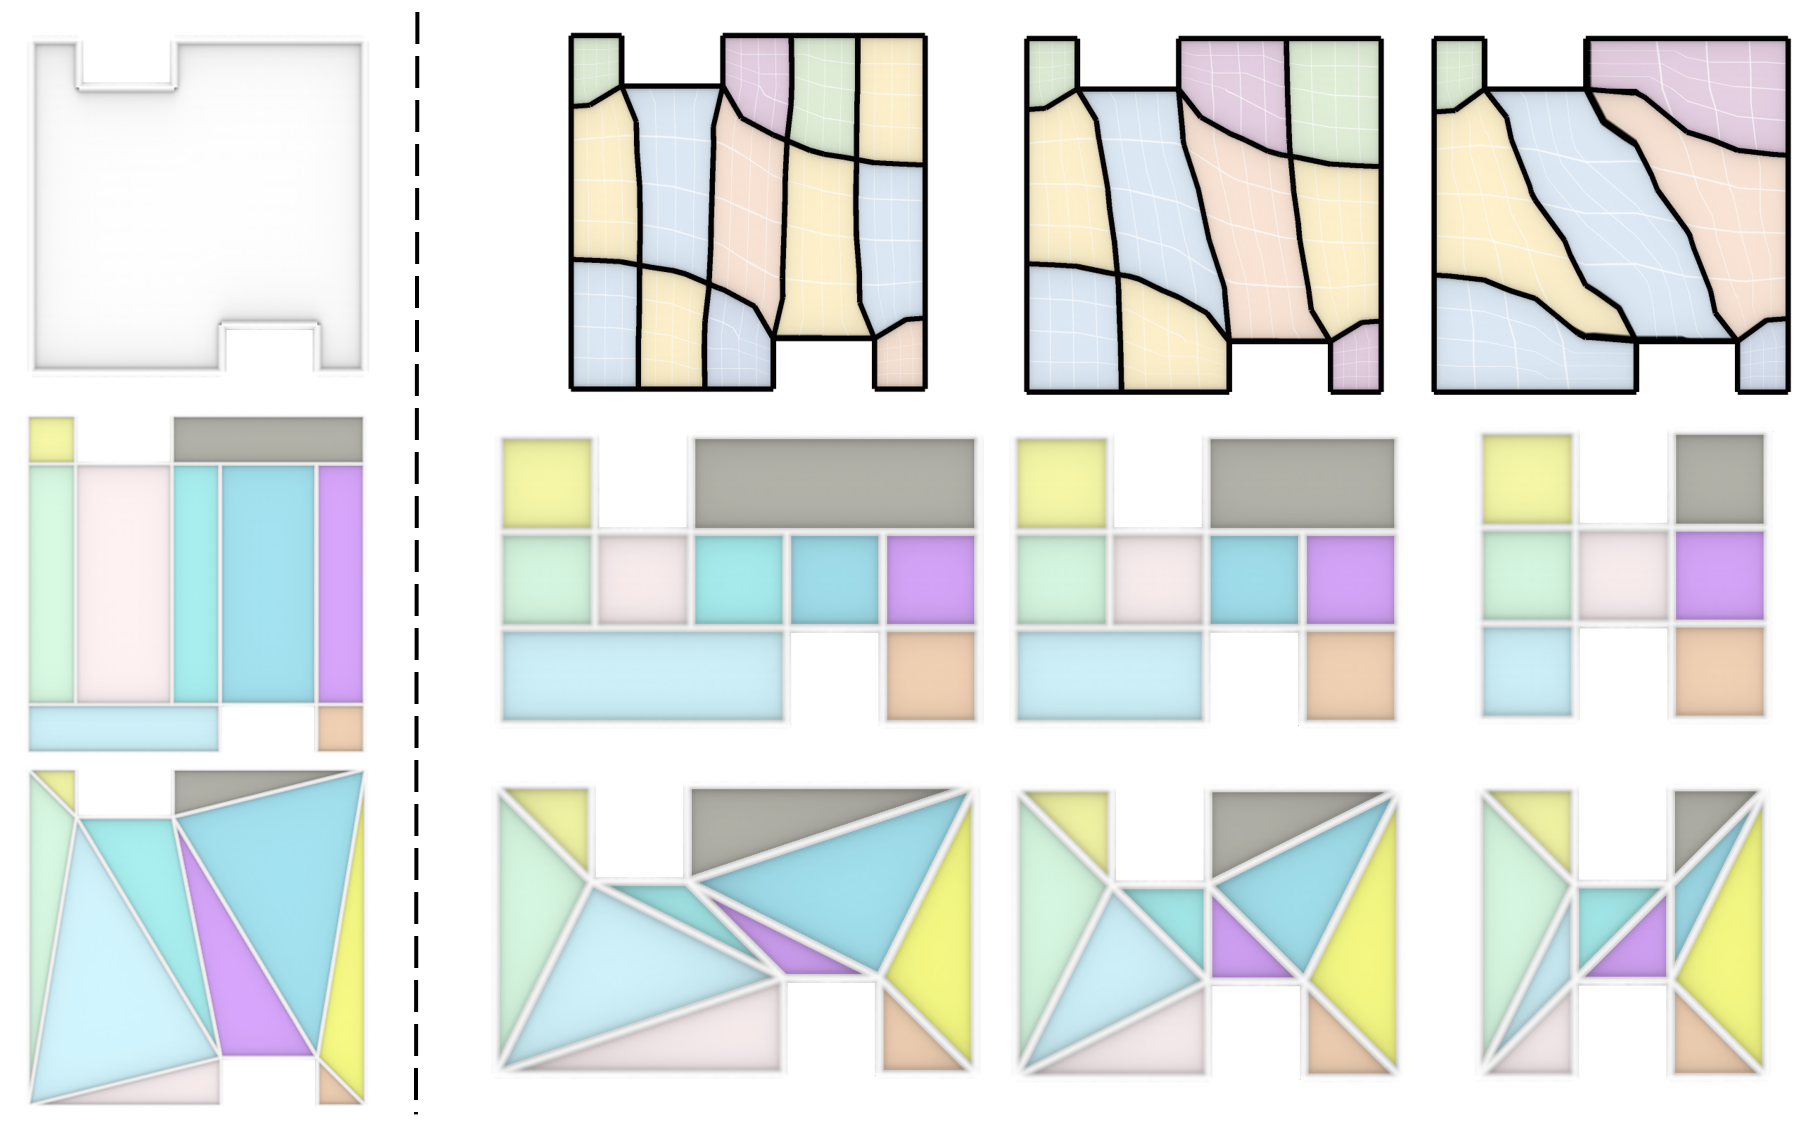
\includegraphics[width=0.8\linewidth]{yoimg/restriction.png}
    \end{itemize}
\end{frame}

\begin{frame}{Résultats}
    \centering
    \includegraphics[width=\linewidth]{yoimg/5_meshes.png}
\end{frame}